%-------------------------------------
% This template comes from Clara Eleonore Pavillet. 

% The Beamer Theme has been modified by Dr. Rahul Raoniar to fulfill B.Tech/Master/Ph.D./PostDoc student's Dissertation/Thesis/Proposal requirements.

% Description: I made this unofficial Beamer Template for the Indian Institute of Technology Bombay (IITB). Feel free to use it, modify it, and share it. 

% Thank you note: A huge thanks goes to Clara Eleonore Pavillet for the original template.
%-------------------------------------

\documentclass[aspectratio=169]{beamer}
% Load Packages
\usepackage[utf8]{inputenc}
\usepackage{xcolor}
\usepackage{tikz} 
\usetikzlibrary{positioning,calc}
\usepackage{graphicx}
\usepackage{hyperref}
\usepackage{amsmath}
\usepackage{listings}
\usepackage{fontawesome}
\usepackage[center]{caption}
\usepackage{makecell}
\usepackage{adjustbox}
\usepackage{multirow}
\usepackage{multicol}
\usepackage{xspace} 
\usepackage{etoolbox} % for text size in table
\usepackage{booktabs} % for \midrule and other
\usepackage{pgfgantt} % for Gentt Chart
\usepackage{ragged2e} % Para justificar o texto
\usepackage{graphicx, animate}
\usepackage{cancel}
\usepackage{chngcntr}
\usepackage{pgfplots}
\usepackage{colortbl}
\usepackage{float}
\usepackage{amssymb} % Para o comando \checkmark
\usepackage{enumitem} % Para personalizar o símbolo da lista
\usepackage[table]{xcolor}
\usepackage{booktabs} 
\usepackage{tabularx}
% Define Commands
\newcommand*{\ClipSep}{0.06cm} %To adjust footer logo
\newcommand{\E}{\mathrm{e}\,} %\def\I{e} % used to defined e for exp(x), see later what it should be
\newcommand{\ud}{\mathrm{d}}
\lstset{numbers=left, numberstyle=\tiny, stepnumber=1,firstnumber=1,breaklines=true,
    numbersep=5pt,language=Python,
    stringstyle=\ttfamily,
    basicstyle=\footnotesize, 
    showstringspaces=false
}

% Remove table's caption using the caption package
\captionsetup{labelformat=empty}

% For smaller size bibliography at the end slide
\setbeamerfont{bibliography entry author}{shape=\scshape,size=\tiny}%
\setbeamerfont{bibliography entry title}{shape=\scshape,size=\tiny}
\setbeamerfont{bibliography entry journal}{shape=\scshape,size=\tiny}
\setbeamerfont{bibliography entry note}{shape=\scshape,size=\tiny}

% Numbered items in Bibliography
\setbeamertemplate{bibliography item}{\insertbiblabel}

% -------------------------------------------
% Defining TikZ geometrics 
% -------------------------------------------

% Tikz library
\usepackage{tikz}
\usetikzlibrary{shapes.geometric, arrows}
\usetikzlibrary{angles,quotes} % Carrega a biblioteca de ângulos
\usetikzlibrary{babel, quotes,angles}
% Defining Tickz Style
\tikzstyle{startstop} = [rectangle, rounded corners, minimum width=3cm, minimum height=1cm, text centered, draw=black, fill=red!40]

\tikzstyle{startstop1} = [rectangle, rounded corners, minimum width=3cm, minimum height=1cm, text centered, draw=black, fill=pink!30]

\tikzstyle{startstop2} = [rectangle, rounded corners, minimum width=3cm, minimum height=1cm, text centered, draw=black, fill=teal!10]

\tikzstyle{io} = [trapezium, trapezium left angle=70, trapezium right angle=110, minimum width=3cm, minimum height=1cm, text centered, text width = 4.5cm, draw=black, fill=blue!30]

\tikzstyle{process} = [rectangle, minimum width=3cm, minimum height=1cm, text centered, text width = 6cm, draw=black, fill=orange!30]

\tikzstyle{decision} = [diamond, minimum width=3cm, minimum height=1cm, text centered, draw=black, fill=green!30]

\tikzstyle{arrow} = [thick,->,>=stealth]

% Representação do diagrama de blocos
\tikzstyle{block} = [draw, fill=blue!20, rectangle, 
    minimum height=3em, minimum width=6em]
\tikzstyle{sum} = [draw, fill=blue!20, circle, node distance=1cm]
\tikzstyle{input} = [coordinate]
\tikzstyle{output} = [coordinate]
\tikzstyle{pinstyle} = [pin edge={to-,thin,black}]

% Ajustes de estilo para as referências
\setbeamerfont{bibliography item}{size=\tiny}
\setbeamerfont{bibliography entry author}{size=\tiny}
\setbeamerfont{bibliography entry title}{size=\tiny}
\setbeamerfont{bibliography entry location}{size=\tiny}
\setbeamerfont{bibliography entry note}{size=\tiny}





\usetheme{oxonian}

% Title page
\title{\textbf{\textcolor{purple}{\LARGE COMPARAÇÃO ENTRE O CONTROLE PID E MPC}}}

% Sub-title
\subtitle{ UM ESTUDO DE CASO COM \textit{CART POLE} E \textit{LUNAR LANDER}}

\titlegraphic{
\includegraphics[width=4.0cm]{Theme/Logos/UFSJ_logo.jpg}}

\author{\footnotesize \textbf{\textcolor{blue}{Gabriel Bueno Leandro}} \newline Orientador \newline \textbf{\textcolor{blue}{Samir Ângelo Milani Martins \vspace{4mm}}}}

\institute{\footnotesize \textbf{Universidade Federal de São João del-Rei
}\\ \vspace{1mm} Departamento de Engenharia Elétrica}

\date{\tiny 9 de abril de 2024} %\today

\begin{document}

{\setbeamertemplate{footline}{} 
\frame{\titlepage}}

%%%%%%%%%%%%%%%%%%%%%%%%%%%%%%%%%%%%%%%%
% Outline
\section*{Outline}
\begin{frame}
    {\textcolor{blue}{\textbf{Esboço da Apresentação}}}\tableofcontents
\end{frame}

%%%%%%%%%%%%%%%%%%%%%%%%%%%%%%%%%%%%%%%%
% Section: Introduction 
%%%%%%%%%%%%%%%%%%%%%%%%%%%%%%%%%%%%%%%%
\section{\textbf{\textcolor{purple}{Introdução}}}
    \begin{frame}[plain]
        \vfill
      \centering
      \begin{beamercolorbox}[sep=8pt,center,shadow=true,rounded=true]{title}
        \usebeamerfont{title}\insertsectionhead\par%
        \color{oxfordblue}\noindent\rule{10cm}{1pt}
      \end{beamercolorbox}
      \vfill
  \end{frame}

%---------------------------------------
% Slide: Motivation of The Study
%---------------------------------------
\begin{frame}{\textcolor{blue}{\textbf{Motivação do estudo}}}
    \vspace{-0.75cm}
    \begin{block}{\textbf{\textcolor{teal}{Importância no contexto da Engenharia}}}
    \begin{itemize}[label={\tikz{\draw[blue,fill=blue,rotate=-90] (0,0) -- (0.2,0) -- (0.1,0.2) -- cycle;}}]
        \justifying % justifica o texto
        \item O controlador PID é, atualmente, o mais prevalente e amplamente adotado nas malhas fechadas industriais \cite{deulkar2020analysis};
        \item  A ISA considera que o controle preditivo é uma ferramenta importante capaz de diferenciar entre um bom e um excelente Engenheiro de Controle;
        \item O Controle Preditivo Generalizado (GPC) emerge como a técnica mais amplamente reconhecida no contexto do Controle Preditivo Baseado em Modelo (MPC) \cite{alba2000control};
        \item O desafio apresentado pelo pêndulo invertido (\textit{Cart Pole}) é um clássico na engenharia de controle;
        \item Estudar os desafios do pouso lunar por meio da simulação no \textit{Lunar Lander} permite entender um pouco sobre autonomia de veículos/robôs.
    \end{itemize}
    \end{block}
\end{frame}
 

%%%%%%%%%%%%%%%%%%%%%%%%%%%%%%%%%%%%%%%%
% Section: Study Objectives 
%%%%%%%%%%%%%%%%%%%%%%%%%%%%%%%%%%%%%%%%
\section{\textbf{\textcolor{purple}{Conceitos Preliminares}}}
    \begin{frame}[plain]
        \vfill
      \centering
      \begin{beamercolorbox}[sep=8pt,center,shadow=true,rounded=true]{title}
        \usebeamerfont{title}\insertsectionhead\par%
        \color{oxfordblue}\noindent\rule{10cm}{1pt}
      \end{beamercolorbox}
      \vfill
  \end{frame}

%---------------------------------------
% Slide: Study Objectives
%---------------------------------------
\begin{frame}{\textcolor{blue}{\textbf{Controlador PID}}}
\vspace{-0.35cm}
Um controlador PID é composto por três termos ajustáveis que atuam em torno do erro do sistema:

\begin{equation}
    \label{eq:erro}   % Nome da equação para referência cruzada
        e(t) = r(t) - y_m(t).
\end{equation}

\begin{equation}% Pid padrão isa    
     \label{eq:pidisa}
        g(t) = K_C\bigg{(}\textcolor{violet}{e(t)} + \textcolor{blue}{\frac{1}{\tau_I}\cdot \int_0^t e(t) dt} +\textcolor{red}{\tau_D \cdot \frac{de(t)}{dt}}\bigg{)}.
\end{equation}

\begin{figure}
\centering
\vspace*{-.45cm}
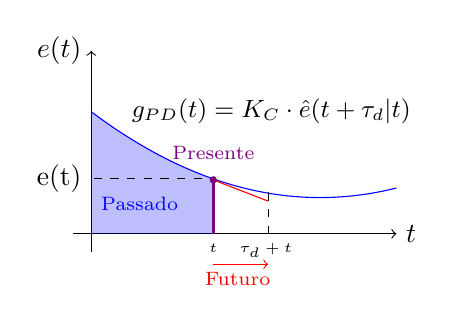
\begin{tikzpicture}[scale=1.55]
    % Eixos
    \draw[->] (-0.15,0) -- (2.5,0) node[right] {$t$};
    \draw[->] (0,-0.15) -- (0,1.5) node[left] {$e(t)$};
    
    % Função
    \draw[domain=0:2.5,smooth,variable=\x,blue] plot ({\x},{0.2*\x^2 - 0.75*\x + 1});
    \draw[domain=0.999:1.45,smooth,variable=\x,red] plot ({\x},{-0.388*\x + 0.83});    
    % Área sob a curva
    \fill[blue, opacity=0.25, domain=0:1, variable=\x]
        (0,0)
        -- plot ({\x}, {0.2*\x^2 - 0.75*\x + 1})
        -- (1,0)
        -- cycle;
    
    % Retângulo
    \draw[dashed] (1,0) -- (1,{0.2*1^2 - 0.75*1 + 1}) -- (0,{0.2*1^2 - 0.75*1 + 1})node[left]{e(t)};
    
    % Etiquetas
    \draw[fill=violet, color=violet] (1, 0.442) circle (0.025cm);
    \draw[color=violet, line width=1pt] (1, 0.442) -- (1, 0);
    \draw[->, color=red] (1, -0.25) -- (1.45, -0.25);
    \node[above, color=violet] at (1,0.525){\scriptsize Presente};
    \node[above, color=red] at (1.2,-0.5){\scriptsize Futuro};
    \draw (1,0) node[below] {\tiny $t$};
    \draw[dashed] (1.45,0) -- (1.45,{0.2*1.35^2 - 0.75*1.35 + 1});
    \draw (1.43,0) node[below] {\tiny $\tau_d+t$};
    \draw (1,{0.2*1^2 - 0.75*1 + 1});% node[left] {$f(a)$};
    \node[right, color=blue] at (0,.25) {\scriptsize Passado};
    %\node[color=red] at (1.22,0.15) {\scriptsize $\frac{de(t)}{dt}$};
    \node[color=black] at (1.475,1) {\small $g_{PD}(t) = K_C\cdot\hat{e}(t+\tau_d|t)$};
    %\draw (0.5,0.5) node {$f(x)$};
    
    % Integral
    %\draw[thick,black] (0,0) -- (1,0);
    %\draw[thick,black] (1,0) -- (1,{0.2*1^2 - 0.5*1 + 1});
    %\draw[thick,black] (0,0) -- (0,{0.2*1^2 - 0.5*1 + 1});
    
    % Label da integral
    %\draw (0.5,1) node[red] {$\int_a^b f(x)\,dx$};
\end{tikzpicture}
\end{figure}
    
\end{frame}

%---------------------------------------
% Slide: Study Methodology 
%---------------------------------------

\begin{frame}
  \frametitle{\textcolor{blue}{\textbf{Controle Preditivo Baseado em Modelo}}}
  
  \begin{itemize}[label={\tikz{\draw[blue,fill=blue,rotate=-90] (0,0) -- (0.2,0) -- (0.1,0.2) -- cycle;}}]
  	\item Trajetória de referência;
  	\item Modelo do processo;
  	\item Otimizador;
  	\item Processo real. 
  \end{itemize}
  
 O Controle Preditivo Generalizado (GPC) se baseia em modelos paramétricos.

\begin{figure}[H]
    \centering
    \vspace*{-0.2cm}
    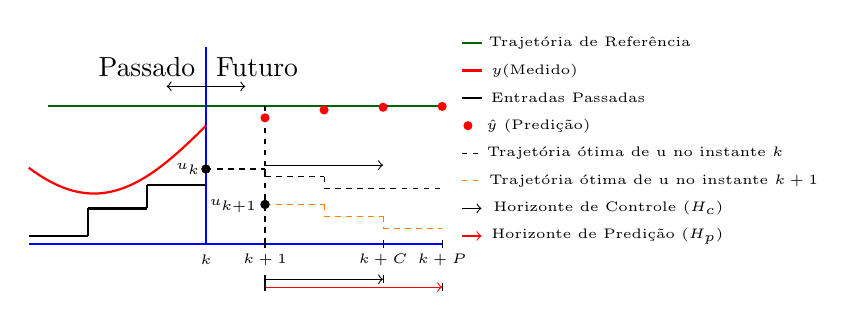
\begin{tikzpicture}
\definecolor{darkgreen}{RGB}{0,100,0}
\draw[color=blue, thick] (-2.25,0) -- (3,0);
\draw[color=darkgreen, thick] (-2,1.75) -- (3,1.75);
\draw[color=blue, thick] (0,0) -- (0,2.5);
\draw[->](0,2)--(0.5,2)node[pos=1.3, above] {Futuro};
\draw[->](0,2)--(-0.5,2)node[pos=1.5, above] {Passado};
\draw[domain=-2.25:0, smooth, samples=100, thick, red] plot (\x, {1.65+sin(\x r)-0.15*cos(\x r)}) node[below right] {};
\draw[thick] (-2.25,0.1) -- (-1.5,0.1);
\draw[thick] (-1.5,0.1)--(-1.5,0.45);
\draw[thick] (-1.5,0.45)--(-0.75,.45);
\draw[thick] (-.75,0.45)--(-.75,0.75);
\draw[thick] (-.75,0.75)--(0,0.75);
\node[font=\tiny] at (0, -0.2) {$k$};
\node[font=\tiny] at (0.75, -0.2) {$k+1$};
\draw(0.75,0.05)--(0.75,-0.05);
\node[font=\tiny] at (2.25, -0.2) {$k+C$};
\draw(2.25,0.05)--(2.25,-0.05);
\node[font=\tiny] at (3, -0.2) {$k+P$};
\draw(3,0.05)--(3,-0.05);
\filldraw[fill=black, draw=black] (0,0.95) circle (.05);
\node[font=\tiny] at (-0.225, 0.95) {$u_k$};
\node[font=\tiny] at (0.35, 0.475) {$u_{k+1}$};
\filldraw[fill=black, draw=black] (0.75,0.5) circle (.05);
\draw[dash pattern=on 2pt off 2pt,color=orange](0.75,0.5)--(1.5,0.5);
\draw[dash pattern=on 2pt off 2pt](0,0.95)--(0.75,0.95);
\draw[dash pattern=on 2pt off 2pt,color=orange](1.5,0.35)--(2.25,0.35);
\draw[dash pattern=on 2pt off 2pt,color=orange](1.5,0.5)--(1.5,0.35);
\draw[dash pattern=on 2pt off 2pt,color=orange](2.25,0.2)--(3,0.2);
\draw[dash pattern=on 2pt off 2pt,color=orange](2.25,0.35)--(2.25,0.2);
\draw[dash pattern=on 2pt off 2pt](0.75,0.95)--(0.75,0.85);
\draw[dash pattern=on 2pt off 2pt](0.75,0.85)--(1.5,0.85);
\draw[dash pattern=on 2pt off 2pt](1.5,0.85)--(1.5,0.7);
\draw[dash pattern=on 2pt off 2pt](1.5,0.7)--(3,0.7);
\draw[dash pattern=on 2pt off 2pt](0.75,0)--(0.75,1.75);
\filldraw[fill=red, draw=red] (0.75,1.6) circle (.05);
\filldraw[fill=red, draw=red] (1.5,1.7) circle (.05);
\filldraw[fill=red, draw=red] (2.25,1.735) circle (.05);
\filldraw[fill=red, draw=red] (3,1.745) circle (.05);
\filldraw[fill=black, draw=black] (0,0.95) circle (.05);
\filldraw[fill=black, draw=black] (.75,0.5) circle (.05);
\draw[color=darkgreen, thick] (3.25,2.55) -- (3.5,2.55)node[pos=6.5,black,font=\tiny]{Trajetória de Referência};
\draw[color=red, thick] (3.25,2.2) -- (3.5,2.2)node[pos=3.7,black, font=\tiny]{$y $(Medido)};
\draw[color=black, thick] (3.25,1.85) -- (3.5,1.85)node[pos=5.4,black,font=\tiny]{Entradas Passadas};
\filldraw[fill=red, draw=red] (3.3275,1.5) circle (.05);
\node[font=\tiny] at (4.225, 1.5) {$\hat{y}$ (Predição)};
\draw[dash pattern=on 2pt off 2pt](3.25,1.15)--(3.5,1.15)node[pos=8.8,black,font=\tiny]{Trajetória ótima de u no instante $k$};
\draw[dash pattern=on 2pt off 2pt,color=orange](3.25,.8)--(3.5,.8)node[pos=9.75,black,font=\tiny]{Trajetória ótima de u no instante $k+1$};
\draw[->](3.25,.45) -- (3.5,.45)node[pos=7.45,black,font=\tiny]{Horizonte de Controle ($H_c$)};
\draw[->,color=red](3.25,0.1) -- (3.5,0.1)node[pos=7.4,black,font=\tiny]{Horizonte de Predição ($H_p$)};
\draw[->](0.75,-.45) -- (2.25,-.45);
\draw[->](0.75,1) -- (2.25,1);
\draw[->, color=red](0.75,-0.55) -- (3,-0.55);
\draw (0.75,-0.4)--(0.75,-0.6);
\draw (2.25,-0.4)--(2.25,-0.5);
\draw (3,-0.5)--(3,-0.6);
\end{tikzpicture}
\label{fig:GCPBM}
\end{figure}
\vspace*{.5cm}

\end{frame}


%---------------------------------------
% Slide: Study Area Map
%---------------------------------------

\begin{frame}{\textcolor{blue}{\textbf{Algoritmos de Otimização}}}

\begin{columns}
\column{0.5\textwidth}
\textcolor{teal}{\textbf{Método de pesquisa em grade}}

\begin{itemize}[label={\tikz{\draw[blue,fill=blue,rotate=-90] (0,0) -- (0.2,0) -- (0.1,0.2) -- cycle;}}]
	\item Complexidade O(n!);
	\item Mínimo/máximo global.
\end{itemize}


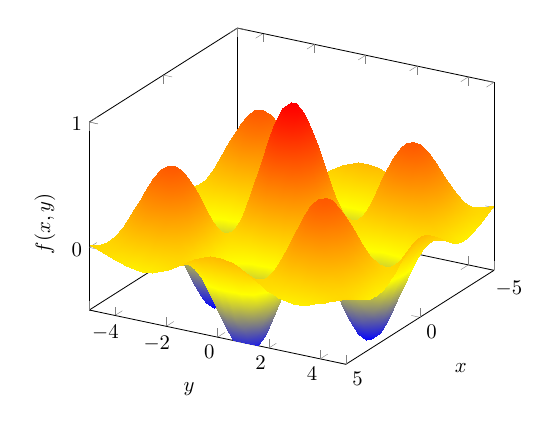
\begin{tikzpicture}[scale=0.75]
\begin{axis}[
    xlabel={$x$},
    ylabel={$y$},
    zlabel={$f(x,y)$},
    xmin=-5, xmax=5,
    ymin=-5, ymax=5,
    zmin=-0.5, zmax=1.0,
    domain=-5:5,
    samples=50,
    view={120}{30}
]

% Função
\addplot3 [surf,shader=interp] {cos(deg(x))*cos(deg(y))*exp(-(x^2 + y^2)/35)};


\end{axis}
\end{tikzpicture}
 

\column{0.53\textwidth}
\vspace*{-3.05cm}

\textcolor{teal}{\textbf{Algoritmo subida de encosta}}
\begin{itemize}[label={\tikz{\draw[blue,fill=blue,rotate=-90] (0,0) -- (0.2,0) -- (0.1,0.2) -- cycle;}}]
	\item Inicialização com uma solução inicial;
	\item \justifying Mover-se iterativamente para uma solução vizinha mais favorável;
	\item \justifying Continuar até não haver mais melhorias ou um critério de parada ser alcançado.
\end{itemize}

\end{columns}

\end{frame}
%---------------------------------------
% Slide: Study Area Map
%---------------------------------------

\begin{frame}{\textcolor{blue}{\textbf{Ambientes}}}
\begin{columns}
\column{0.5\textwidth}
\textbf{\textcolor{teal}{\textit{Cart Pole}}}

\begin{figure}[H]
    \centering
    \vspace*{-0.25cm}
    \animategraphics[width=.55\textwidth, loop, autoplay]{50}%frame rate
    {images/CPSC.png/10064094-80f5-4740-bbfb-425e476c87c0-}%path to figures
    {0}%start index
    {24}%end index
    \label{fig:GPC1}
\end{figure}

\begin{table}[H]
    \centering
    \vspace*{-0.2cm}
    \LARGE % Tamanho da fonte reduzido
    \resizebox{\columnwidth}{!}{%
        \begin{tabular}{cccc}
            \rowcolor{blue!30} Número & Observação & Mínimo & Máximo  \\
 			\hline
            0 & Posição & -4,8 & 4,8\\
            1 & Velocidade linear & -Inf & Inf\\
            2 & Ângulo & $-0,418$ rad ($-24^\circ$) & $0,418$ rad ($24^\circ$)\\
            3 & Velocidade angular & -Inf & Inf\\
            \hline
        \end{tabular}  
    }
    \label{tab:outcartpole}
\end{table}
\vspace*{1.25cm}
\column{0.5\textwidth}
 \vspace*{-.05cm}
\textbf{\textcolor{teal}{\textit{Lunar Lander}}}

\begin{figure}[H]
    \centering
     \vspace*{-.05cm}
    \animategraphics[width=.625\textwidth, loop, autoplay]{45}%frame rate
    {images/LLSC.png/1d08ba8c436d45c4836197d017e10367pXCEhE5SPawIdiCa-}%path to figures
    {0}%start index
    {118}%end index
    \label{fig:GPC1}
\end{figure}

\begin{table}[H]
	\centering
	\vspace*{-1.075cm}
    \small % Tamanho da fonte reduzido
    \resizebox{\columnwidth}{!}{%
        \begin{tabular}{cccc}
            \rowcolor{blue!30} Número & Observação & Mínimo & Máximo  \\
            \hline
            0 & Coordenada x & -1,5 & 1,5\\
            1 & Coordenada y & -1,5 & 1,5\\
            2 & Velocidade linear em x &  -5 & 5\\
            3 & Velocidade linear em y &  -5 & 5\\
            4 & Ângulo & -$\pi$  $(-180^\circ)$ & $\pi$ $(180^\circ)$\\
            5 & Velocidade angular &  -5 & 5\\
            6 & Contato pé esquerdo &  0 & 1\\
            7 & Contato pé direito &  0 & 1\\
        \hline
        \end{tabular}
        }
        \label{tab:outlunarlander}                 % Nome da tabela para referência cruzada
    \end{table}

\end{columns}
\end{frame}

%%%%%%%%%%%%%%%%%%%%%%%%%%%%%%%%%%%%%%%%
% Section: Modeling 
%%%%%%%%%%%%%%%%%%%%%%%%%%%%%%%%%%%%%%%%
\section{\textbf{\textcolor{purple}{Metodologia}}}
    \begin{frame}[plain]
        \vfill
      \centering
      \begin{beamercolorbox}[sep=8pt,center,shadow=true,rounded=true]{title}
        \usebeamerfont{title}\insertsectionhead\par%
        \color{oxfordblue}\noindent\rule{10cm}{1pt}
      \end{beamercolorbox}
      \vfill
  \end{frame}

%---------------------------------------
% Slide: Modeling Framework
%---------------------------------------

\begin{frame}{\textcolor{blue}{\textbf{Obtenção da Função de Transferência \textit{Cart Pole}}}}
\begin{columns}
\column{0.5\textwidth}
\begin{figure}
\vspace*{-0.475cm}
\centering
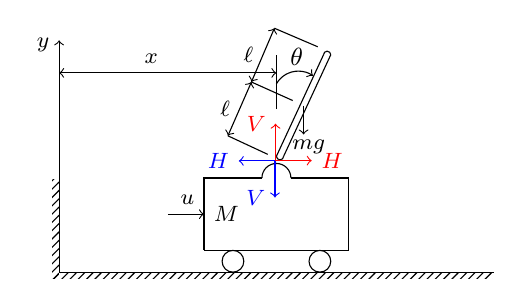
\begin{tikzpicture}[scale=.92, every node/.style={font=\footnotesize}]
    \draw[pattern=north east lines, pattern color=black,  draw=white] (-0.1,0) rectangle (6,-0.1);
    \draw[pattern=north east lines, pattern color=black,  draw=white] (-0.1,-0.1) rectangle (0,1.3);
    \draw (0,0) -- (6,0);
    \draw (0,0) -- (0,1.3);
    \draw (2.4, 0.15) circle (0.15cm);
    \draw (3.6, 0.15) circle (0.15cm);
    \draw (2,0.3) -- (4,0.3) -- (4,1.3) -- (3.2,1.3);
    \draw(2.8,1.3)--(2,1.3)--node[right]{$M$}(2,0.3);
    \draw (3.2,1.3) arc (0:180:0.2cm);
    \draw (3, 1.6)--(3.65, 3);
    \draw (3.1, 1.6)--(3.75, 3);
    \draw (3.1,1.6) arc (0:-180:0.05cm);
    \draw (3.75,3) arc (0:180:0.05cm);
    \draw[->](0,2.6)--node[above left]{$y$}(0,3.2);
    \draw(0,1.3)--(0,2.6);
    \draw (3, 2.25)--(3,3);
    \draw [<->] (0, 2.75)--node[above left]{$x$}(3, 2.75);
    \draw [->](3,2.6) arc (150:55:0.35cm) node[above left]{\small $\theta$};
    \draw[->](3.375,2.3)--node[pos=2, above]{$\:\:mg$}(3.375,1.9);
    \draw[->] (1.5,0.8) -- (2,0.8) node[above left] {$u$};
    %\draw (3.03, 1.557)--(3.72,3.042);
    %\draw (2.88, 1.626)--(3.57,3.111);
    \draw (2.655,2.6248)--(3.225,2.3688);
    \draw [<->](2.33, 1.882)--node[left]{$\ell$}(2.655,2.6248);
    \draw [<->](2.655,2.6248)--node[left]{$\ell$}(2.972,3.367);
    \draw (3.57,3.111)--(2.972,3.367);
    \draw (2.33, 1.882)--(2.88, 1.626);
    \draw[->, blue] (2.98,1.535) -- (2.48,1.535) node[left] {$H$};
    \draw[->, blue] (2.98,1.535) -- (2.98,1.03) node[left] {$V$};
    \draw[->, red] (2.9875,1.54) -- (2.9875,2.05) node[left] {$V$};
    \draw[->, red] (2.9875,1.54) -- (3.4875,1.54) node[right] {$H$};
\end{tikzpicture}
\label{fig:corpolivre}
%\caption{\justifying Diagrama de corpo livre do sistema de pêndulo invertido}
\end{figure}

\begin{figure}[H]
    \definecolor{lightbrown}{RGB}{205,133,63} % Define a cor marrom claro
    \centering
    \vspace*{-0.25cm}
    \begin{tikzpicture}[scale=.92, every node/.style={font=\footnotesize}]
         % Cartpole 1
        \draw [->](-3, 0) --node[above left]{$y$}(-3, 1);
        \draw [->](-3, 0) --node[above right]{$x$}(-2, 0);
        \draw[fill = lightbrown, rotate around={0:(0,0)}]  (0,0) rectangle (0.1,3);
        \node[circle,fill=green,inner sep=1pt] at (0.05,1.5) {};
        \draw[fill = lightbrown, rotate around={-45:(0,0)}] (0,0) rectangle (0.1,3);
        \node[circle,fill=cyan,inner sep=1pt] at (1.0606,0.986) {};
        \coordinate (A) at (1.13,1);
        \coordinate (B) at (-.2,-.2);
        \coordinate (C) at (0.11,1);
        \draw (-0.1, 0) -- (-1.2,0);
        \draw (-0.1, 1.5) -- (-1.2,1.5);
        \draw [<->, fill=black](-1.15, 0)--node[left]{$\ell$} (-1.15,1.5);
        \draw [<->](0.05, 0.986)--node[above]{$\ell sen\theta$} (1.0606,0.986);
        \draw (-0.1, 0.986) -- (-0.2,0.986);
        \draw [<->](-0.15, 0) --node[left]{$\ell cos\theta$}(-0.15,0.986);
        \draw[dashed] (0.05,1.5) -- (2,1.5); 
        \draw[dashed] (1.0606,0.986) -- (2,0.986); 
        \draw [<->](1.95, 0.986) --node[right]{$\ell - \ell cos\theta$}(1.95, 1.5);
        \pic[draw=black, <->, angle radius=1cm, angle eccentricity=.8]{angle = A--B--C};
        \node at (.225,.5) {$\theta$};
    \end{tikzpicture}
    \label{fig:des}
    %\caption{\justifying Deslocamento do centro de massa do pêndulo}
\end{figure}

\column{0.56\textwidth}
\vspace*{-0.85cm}

Deslocamento horizontal do carro:

\begin{equation}
    \label{eq:hori}
    M\frac{d^2x}{dt} = u - H.
\end{equation}

Equilíbrio das forças horizontais do pêndulo:

\begin{equation}
    m\frac{d^2}{dt}(x+\ell sen\theta) = H\Rightarrow m\frac{d^2}{dt}(x+\ell\theta) = H.
    \label{eq:descmh}
\end{equation}

Equilíbrio das forças verticais do pêndulo:

\begin{equation}
         m\frac{d^2}{dt}(\ell-\ell cos\theta) = m g - V\Rightarrow 0 = V-m g.
    \label{eq:descmv}
\end{equation}

\end{columns}
\end{frame}

%---------------------------------------
% Slide: Modeling Framework
%---------------------------------------

\begin{frame}{\textcolor{blue}{\textbf{Obtenção da Função de Transferência \textit{Cart Pole}}}}
\begin{columns}
\column{0.5\textwidth}
\begin{figure}[H]
    \definecolor{lightbrown}{RGB}{205,133,63} % Define a cor marrom claro
    \centering
    \vspace*{-0.85cm}
    \begin{tikzpicture}[scale=.85,every node/.style={font=\footnotesize}]
        % Cartpole 1
        \draw[rotate around={0:(0,0)}]  (0,1.45) rectangle (0.1,-1.45);
        \draw[fill = lightbrown, rotate around={-45:(0,0)}]  (0,1.5) rectangle (0.1,-1.5);
        \node[circle,fill=blue,inner sep=1pt] at (0.05,0) {};
        \draw [->, red](-1.015, -1.1) --node[above right]{$V$}(-1.015, 0.015);
        \draw [->, red](-1.015, -1.1) --node[above right]{$H$}(-0.015, -1.1);
        \draw [->, orange](-1.015, 0.015) --node[above left]{$V\:cos\theta$}(-1.515, -0.5153);
        \draw [->, orange](-0.015, -1.1) --node[below right]{$H\:sen\theta$}(-0.545, -1.63);
        \draw [->, orange](-1.015,-1.1) --node[below left]{$H\:cos\theta$}(-0.545, -1.63);
        \draw [->, orange](-1.015, -1.1) --node[below left]{$V\:sen\theta$}(-1.515, -0.5153);
    \end{tikzpicture}
    %\caption{\justifying Deslocamento rotacional do centro de gravidade do pêndulo}
    \label{fig:desr}
\end{figure}
\vspace*{-0.25cm}
Movimento rotacional do pêndulo:

\begin{equation}
    I\frac{d^2\theta}{dt} = V\ell sen\theta - H\ell cos\theta,
    \label{eq:rot}
\end{equation}

\noindent ou ainda:

\begin{equation}
    I\frac{d^2\theta}{dt} = V\ell\theta - H\ell.
    \label{eq:rots}
\end{equation}

\column{0.495\textwidth}
\vspace{-.95cm}

\justifying Onde, $H = m\frac{d^2}{dt}(x+\ell\theta)$ e $V = mg$, assim:

\begin{equation}
    I\frac{d^2\theta}{dt} = mg\theta\ell-m\frac{d^2}{dt} (x+\ell\theta)\ell m.
    \label{eq:HeV}
\end{equation}

\justifying Ao igualar a zero, tem-se:

\begin{equation}
    (I + m\ell^2)\frac{d^2\theta}{dt^2} + m\ell\frac{d^2x}{dt^2} - mg\ell\theta = 0.
    \label{eq:HeV0}
\end{equation}

\justifying Substituindo a expressão de $H$ em $M\frac{d^2x}{dt} = u - H$, chega-se:

\begin{equation}
    M\frac{d^2x}{dt^2}  = u -  m\frac{d^2}{dt^2} (x + \ell\theta).
    \label{eq:Id2r}
\end{equation}

\end{columns}
\end{frame}

%---------------------------------------
% Slide: Modeling Framework
%---------------------------------------

\begin{frame}{\textcolor{blue}{\textbf{Obtenção da Função de Transferência \textit{Cart Pole}}}}
\vspace*{-.75cm}
\begin{equation}
    M\frac{d^2x}{dt^2} + m\frac{d^2}{dt^2} (x + \ell\theta) = u.
    \label{eq:Id2r}
\end{equation}

 Ao considerar a transformada de Laplace com condições iniciais nulas:

\begin{equation}
    (I + m\ell^2)s^2\Theta(s) + m\ell s^2 X(s) - mg\ell\Theta(s) = 0,
    \label{eq:L1}
\end{equation}

\begin{equation}
    (M+m)s^2 X(s) + m\ell s^2\Theta(s) = U(s).
    \label{eq:L2}
\end{equation}

Após algumas manipulações, chega-se à FT \cite{ogata2010engenharia}:

\begin{equation}
    \frac{\Theta (s)}{U(s)} = \frac{m\ell}{(m^2\ell^2-(M+m)(I+m\ell^2))s^2+(M+m)mg\ell}.
    \label{eq:TF}
\end{equation}
\end{frame}

%---------------------------------------
% Slide: Modeling Framework
%---------------------------------------

\begin{frame}{\textcolor{blue}{\textbf{Obtenção da Função de Transferência \textit{Cart Pole}}}}
\begin{columns}
\column{0.5\textwidth}
Força constante à direita:
\begin{figure}[H]
     \centering
     \vspace*{0cm}
     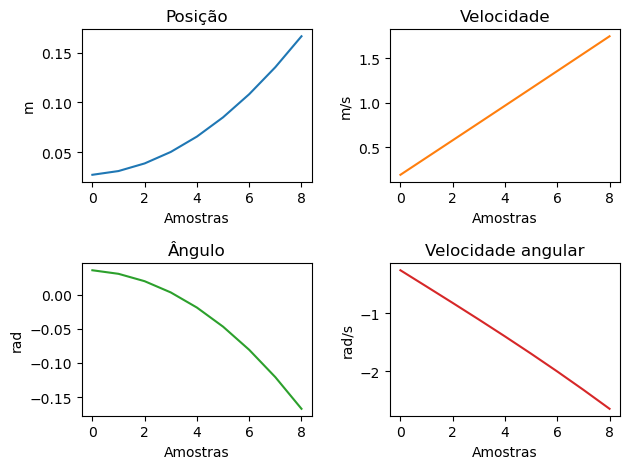
\includegraphics[scale=.475]{images/Grafico1.png}
     \label{fcte}
\end{figure}

\column{0.4\textwidth}
\vspace{-1cm}

Aceleração linear:

\begin{equation}
    \begin{matrix}
        \ddot{x} = 0,19524\frac{m}{s^2}.
    \end{matrix}
\label{eq:vlevt}
\end{equation}

Aceleração angular:

\begin{equation}
    \begin{matrix}
        \ddot{\theta} =-0,29775\frac{rad}{s^2}.
    \end{matrix}
\label{eq:vlevt}
\end{equation}

\end{columns}
\end{frame}


\begin{frame}{\textcolor{blue}{\textbf{Obtenção da Função de Transferência \textit{Cart Pole}}}}
\begin{columns}
\column{0.5\textwidth}
\vspace{-.65cm}

\begin{figure}[H]
	\vspace{0.5cm}
    \definecolor{lightbrown}{RGB}{205,133,63} % Define a cor marrom claro
    \centering    \begin{tikzpicture}[scale=0.8, every node/.style={font=\tiny}]
        % Cartpole 1
        \draw[fill=black] (0,0) rectangle (0.75,0.5);
        \draw[fill=black] (-2,.25) -- (3,.25);
        \draw[fill = lightbrown, rotate around={75:(0.565,0.1)}] (0.5,0.25) rectangle (2,0.385);
        \node[circle,fill=purple,inner sep=1pt] at (0.375,0.25) {};
        \draw [->, blue] (-.5,0.05) -- node[left]{$\Vec{F}$ à direita\:\:}(0, 0.05);
        \coordinate (A) at (.4,.55);
        \coordinate (B) at (.35,.35);
        \coordinate (C) at (0,.55);
        \pic[draw=green, ->, angle radius=1cm,angle eccentricity=.2] {angle = A--B--C};
        %\draw [-, violet] (0.45,1.65) -- node[below left]{$\tau$}(0.45, 1.65);
        \node[color=black] at (1.5,1) {\large $I>0$};
    \end{tikzpicture}
    \label{fig:cartPole}
\end{figure}
\vspace*{-0.25cm}
Considere:

\begin{equation}
    (I + m\ell^2)\frac{d^2\theta}{dt^2} + m\ell\frac{d^2x}{dt^2} - mg\ell\theta = 0.
    \label{eq:an1}
\end{equation}

\justifying Sendo $\theta\approx 0$:

\begin{equation}
    (I + m\ell^2)\frac{d^2\theta}{dt^2}   = - m\ell\frac{d^2x}{dt^2},
    \label{eq:an22}
\end{equation}
\vspace{0.55cm}
\column{0.5\textwidth}
\vspace{-0.75cm}

\noindent numericamente:

\begin{equation}
    I = \frac{0,0976\ell - 0,1488\ell^2}{0,29775}.
    \label{eq:an2}
\end{equation}

\begin{figure}[H]
     \centering
     \vspace*{-.4425cm}
     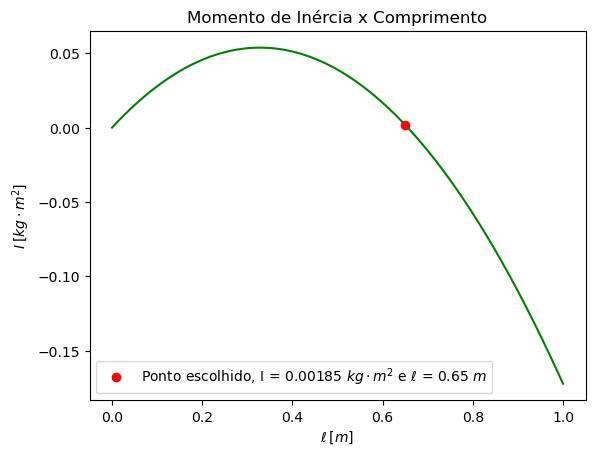
\includegraphics[scale=.45]{images/Grafico2.png}
     \label{fcte}
\end{figure}

\end{columns}
\end{frame}

%---------------------------------------
% Slide: Modeling Framework
%---------------------------------------

\begin{frame}{\textcolor{blue}{\textbf{Obtenção da Função de Transferência \textit{Cart Pole}}}}
\begin{columns}
\column{0.5\textwidth}
\justifying 
Agora, será estimada a massa do carro:

\begin{equation}
    (M + m)\frac{d^2 x}{dt^2} + m\ell \frac{d^2 \theta}{dt^2} = u,
    \label{eq:M}
\end{equation}
\justifying
\noindent isolando $M$:

\begin{equation}
    M = \frac{u - m\ell\ddot{\theta}-m\ddot{x}}{\ddot{x}},
\end{equation}
\justifying
\noindent como $m = 0,5kg$, $u = 1N$ e $\ell = 0,65m$, tem-se:

\begin{equation}
    M  =  5,11754 kg.
\end{equation}
\vspace*{.755cm}
\column{0.5\textwidth}
\justifying Os resultados encontrados/fixados foram:

\begin{table}[H, line width=3.5pt]
\vspace{-.2cm}
	\centering
    \begin{tabular}{cccc}
            \rowcolor{blue!30} $M [kg]$ & $m [kg]$ & $\ell [m]$ & $I[kg\cdot m^2]$\\
            \hline
            $5,11754$ & $0,5$ & $0,65$ & $1,8537\times 10^{-3}$ \\
            \hline
        \end{tabular}
        \label{tab:outlunarlander}                 % Nome da tabela para referência cruzada
 \end{table}

 Ao substituí-los na FT da Equação \ref{eq:TF}, chega-se:

 \begin{equation}
     \frac{\Theta (s)}{U(s)} = \frac{0,325}{-1,0914s^2 + 17,9101}.
    \label{eq:FT1}
\end{equation}

\vspace*{1.4925cm}
\end{columns}
\end{frame}



\begin{frame}{\textcolor{blue}{\textbf{Obtenção da Função de Transferência \textit{Cart Pole}}}}
\begin{columns}
\column{0.5\textwidth}
\vspace{-.55cm}
\begin{figure}[H]
     \centering
     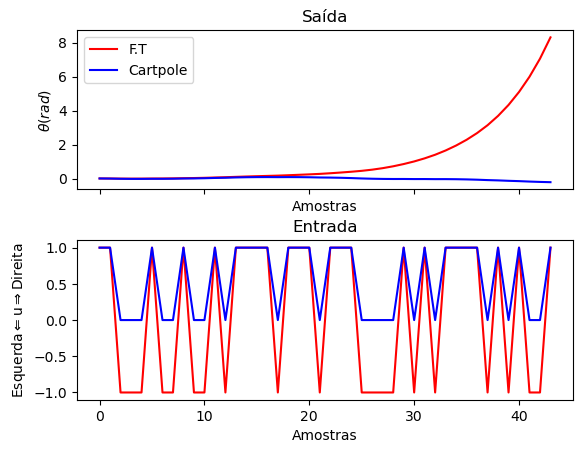
\includegraphics[scale=.45]{images/entval.png}
     \label{fig:entval}
\end{figure}

\justifying A FT não conseguiu representar o sistema adequadamente.
\column{0.52\textwidth}
\justifying As acelerações $\ddot{x}$ e $\ddot{\theta}$ serão multiplicadas por $k$. Considere a Equação de Inércia:

\begin{equation}
    (I + m\ell^2)\frac{d^2\theta}{dt^2}\cancel{k}   = - m\ell\frac{d^2x}{dt^2} \cancel{k}.
    \label{eq:inercia}
\end{equation}

\noindent \justifying $\text{Se} \quad \frac{d\vec{a}}{dt} > 0 \quad \text{e} \quad \vec{F} = \text{cte}, \quad \text{então} \quad \frac{dM}{dt} < 0$:

\begin{equation}
    M = \frac{u - km\ell\ddot{\theta}-km\ddot{x}}{k\ddot{x}}.
    \label{eq:Ma}
\end{equation}
\vspace*{.85cm}
\end{columns}
\end{frame}

%---------------------------------------
% Slide: Modeling Framework
%---------------------------------------

\begin{frame}{\textcolor{blue}{\textbf{Obtenção da Função de Transferência \textit{Cart Pole}}}}
\begin{columns}
\column{0.45\textwidth}
Onde $M > 0$, logo:

\begin{equation}
    0 < \frac{u - km\ell\ddot{\theta}-km\ddot{x}}{k\ddot{x}},
    \label{eq:M>0}
\end{equation}
\hspace{.1cm}
 ou ainda:

\begin{equation}
     0 < 1 + 0,096768k- 0,09762k,
    \label{eq:M>0}
\end{equation}

\noindent \justifying chega-se a $k<1174,74$, o valor de \( k \), ele será variado de 1 a 1174.
\vspace*{.75cm}
\column{0.625\textwidth}
\vspace{-0cm}

\begin{figure}[H]
     \centering
     \vspace*{-1.1cm}
     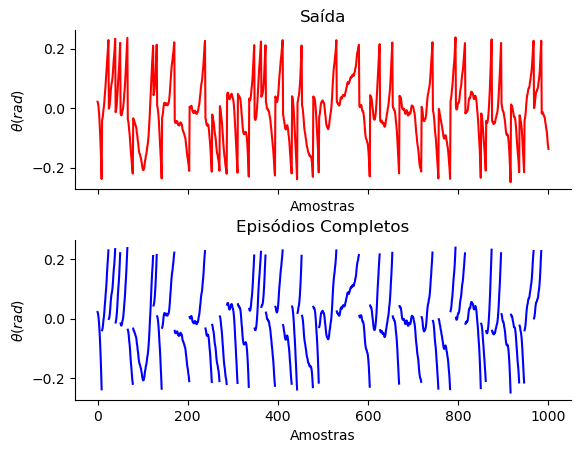
\includegraphics[scale=.42]{images/episodio.png}
     \label{fcte}
\end{figure}
\vspace{-.2cm}
\begin{equation}
    \overline{RMSE}_k = \frac{1}{47} \sum_{ep=1}^{47} \frac{\sqrt{\sum_{i=1}^{N}(y_{ep}(i)-\hat{y}_{ep}(i))^2}}{\sqrt{\sum_{i=1}^{N}(y_{ep}(i)-\bar{y}_{ep})^2}}.
\label{eq:RMSE}
\end{equation}

\end{columns}
\end{frame}

%---------------------------------------
% Slide: Modeling Framework
%---------------------------------------

\begin{frame}{\textcolor{blue}{\textbf{Obtenção da Função de Transferência \textit{Cart Pole}}}}
\begin{columns}
\column{0.5\textwidth}
\vspace{-.55cm}

\begin{figure}[H]
\vspace{-.5cm}
     \centering
     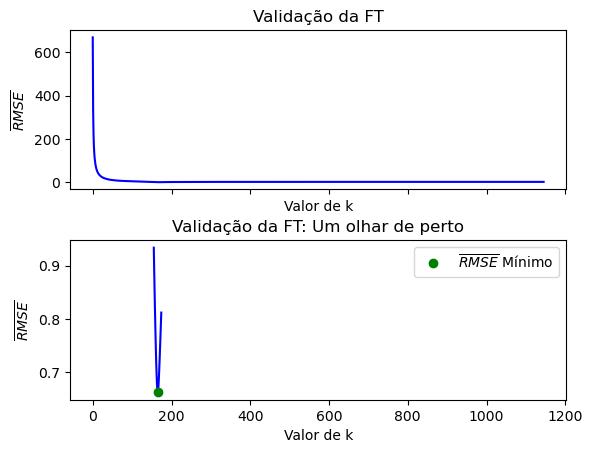
\includegraphics[scale=.475]{images/RMSE1.png}
     \label{fcte}
\end{figure}
\vspace{-.85cm}
\justifying Ao tomar $k=165$, obtém-se uma FT que responde melhor aos estímulos da entrada.

\column{0.5\textwidth}
\vspace{-.75cm}

A nova massa passa a ser:

\begin{equation}
    M = 0,02668 kg,
    \label{eq:MV}
\end{equation}

\noindent \justifying com os novos valores dos parâmetros, a FT passa a ser:

\begin{equation}
     \frac{\Theta (s)}{U(s)} = \frac{0,325}{-0,00661s^2 +  1,67919}.
    \label{eq:31}
\end{equation}


\begin{figure}[H]
\centering
\vspace*{-.475cm}
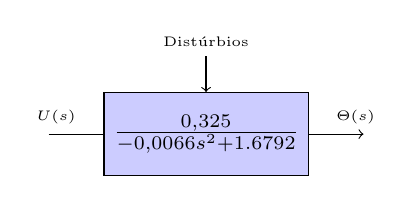
\begin{tikzpicture}[scale=0.8, auto, node distance=2cm]
    % We start by placing the blocks
    \node [input, name=input] {};
    \node [block] (system){};
    \draw [->] (-2.5,0) -- node[above left]{\tiny $U(s)$} (system);
    \draw [->] (system) -- node[above right]{\tiny $\Theta (s)$} (2.5,0);
    \node [block, pin={[pinstyle]above:\tiny Distúrbios},
    node distance=3cm] (system) {$\frac{0,325}{-0,0066s^2 +  1.6792}$};
\end{tikzpicture}
\label{blocos}
\end{figure}

\end{columns}
\end{frame}

%---------------------------------------
% Slide: Modeling Framework
%---------------------------------------

\begin{frame}{\textcolor{blue}{\textbf{Sintonia do PID}}}
\vspace*{-.6cm}
\justifying Para estabilizar o sistema, será utilizado um controlador PID:

\begin{figure}[H]
\centering
\vspace*{-.255cm}
% The block diagram code is probably more verbose than necessary
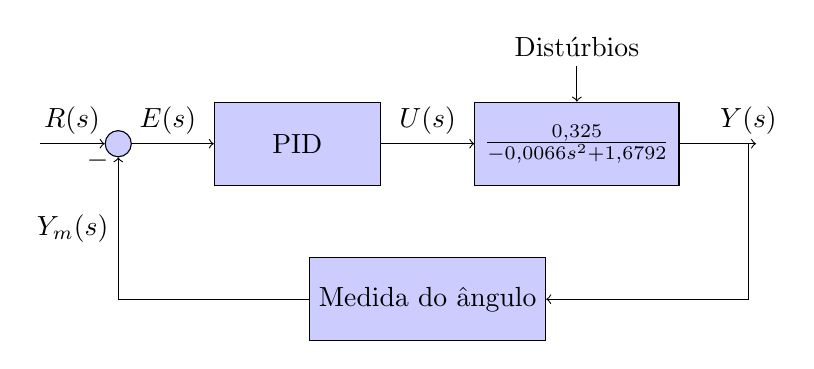
\begin{tikzpicture}[auto, node distance=2.275cm]
    % We start by placing the blocks
    \node [input, name=input] {};
    \node [sum, right of=input] (sum) {};
    \node [block, right of=sum] (controller) {PID};
    \node [block, right of=controller, pin={[pinstyle]above:Distúrbios},
            node distance=3.55cm] (system) {$\frac{0,325}{-0,0066s^2 +  1,6792}$};
    % We draw an edge between the controller and system block to 
    % calculate the coordinate u. We need it to place the measurement block. 
    \draw [->] (controller) -- node[name=u] {$U(s)$} (system);
    \node [output, right of=system] (output) {};
    \node [block, below of=u] (measurements) {Medida do ângulo};

    % Once the nodes are placed, connecting them is easy. 
    \draw [draw,->] (input) -- node {$R(s)$} (sum);
    \draw [->] (sum) -- node[pos=0.44] {$E(s)$} (controller);
    \draw [->] (system) -- node [name=y, pos=0.9] {$Y(s)$}(output);
    \draw [->] (y) |- (measurements);
    \draw [->] (measurements) -| node[pos=0.99] {$-$} 
        node [near end] {$Y_m(s)$} (sum);
\end{tikzpicture}
\end{figure}
\vspace*{-.4cm}
\justifying Considere a expressão do PID:

\begin{equation}
     g(t) = K_C \cdot e(t) + \frac{K_C}{\tau_I}\cdot \int_0^t e(t) dt + K_C\cdot \tau_D \cdot \frac{de(t)}{dt},
    \label{eq:tempopid}
\end{equation}

 o $\tau_i$ foi fixado em 2 e $\tau_d$ em 0,25.

\end{frame}


%---------------------------------------
% Slide: Modeling Framework
%---------------------------------------

\begin{frame}{\textcolor{blue}{\textbf{Sintonia do PID}}}
\vspace*{-.6cm}
\justifying O pacote GEKKO \cite{gekko} fornecerá o valor de $K_C$ ao minimizar:

\begin{equation}
     e(t) = r(t) - y_m(t).
    \label{eq:erro}
\end{equation}

Os parâmetros encontrados foram:

 \begin{table}[H]
	\centering
	\vspace*{-0.05cm}
        \begin{tabular}{ccc} % Defina o formato da sua tabela
            \rowcolor{blue!30} Termos & Relação com $K_C$ & Valor \\
            \hline
            Proporcional & $K_C$ & 0,5 \\
            Integral & $\frac{K_C}{\tau_I}$ & 0,25 \\
            Derivativo & $K_C \cdot \tau_D$ & 0,125 \\
            \hline
        \end{tabular}
        \label{tab:outlunarlander}                 % Nome da tabela para referência cruzada
    \end{table}

\justifying Ao substituir os valores, obtém-se:

\begin{equation}
     g(t) = 0,5 \cdot e(t) + 0,25\cdot \int_0^t e(t) dt + 0,125 \cdot \frac{de(t)}{dt}.
    \label{eq:tempopidv}
\end{equation}

\end{frame}

%---------------------------------------
% Slide: Modeling Framework
%---------------------------------------

\begin{frame}{\textcolor{blue}{\textbf{Sintonia PID}}}
\begin{columns}
\column{0.52\textwidth}
\vspace{-1.15cm}

\justifying A expressão completa para o controlador PID é:

\begin{equation}
     u_n = 0,5 \cdot \theta_n + 0,25\cdot \sum_{i=0}^n \theta_i + 0,125 \cdot \omega_n.
    \label{eq:39}
\end{equation}

\justifying É fundamental realizar uma análise gráfica da saída do GEKKO.

\column{0.5\textwidth}
\vspace{-0.7625cm}

\begin{figure}[H]
\vspace{.2cm}
     \centering
     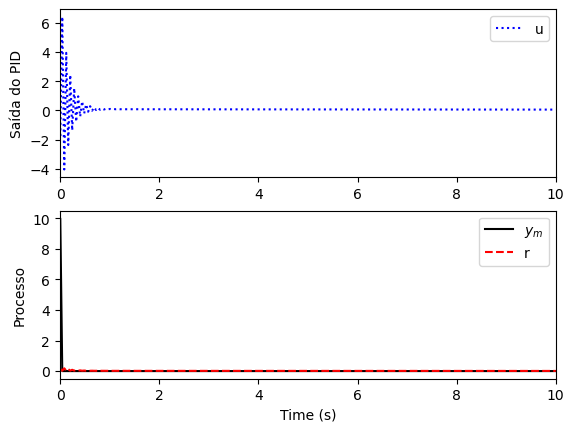
\includegraphics[scale=.5]{images/pid.png}
     \label{fcte}
\end{figure}

\end{columns}
\end{frame}

%---------------------------------------
% Slide: Modeling Framework
%---------------------------------------

\begin{frame}{\textcolor{blue}{\textbf{GPC: Formulação para o \textit{Cart Pole}}}}
\vspace{-.5cm}
\justifying O primeiro passo é definir a trajetória de referência:

\begin{equation}
    w = [0,\:0,\:0, \cdots,\:n_{etapas}].
    \label{eq:traref}
\end{equation}

\justifying Sendo a Função Custo utilizada:

\begin{equation}
    J(k) =\sqrt{(\sum_{j=d}^{h_p} [\hat{y}(j+k|k) - w(j+k)])^2}.
    \label{eq:FO}
\end{equation}

\justifying Deve-se também, definir todos os $\Delta u$ possíveis, logo:

\begin{equation}
    \begin{matrix}
        u_{k-1} = 1 \text{ e } u_{k} = -1 \Rightarrow \Delta u = -2 \\
        u_{k-1} = 1 \text{ e } u_{k} = 1 \Rightarrow \Delta u = 0\\
        u_{k-1} = -1 \text{ e } u_{k} = -1 \Rightarrow \Delta u = 0\\
        u_{k-1} = -1 \text{ e } u_{k} = 1 \Rightarrow \Delta u = 2 \\
    \end{matrix}.
\end{equation}

\end{frame}

%---------------------------------------
% Slide: Modeling Framework
%---------------------------------------

\begin{frame}{\textcolor{blue}{\textbf{GPC: Formulação para o \textit{Cart Pole}}}}
\vspace{-.5cm}

\justifying A definição do problema de otimização é a seguinte:

\begin{equation}
    \begin{matrix}
        \textbf{Minimizar} & J(k) =\sqrt{(\sum_{j=d}^{h_p} [\hat{y}(j+k|k) - w(j+k)])^2}\\
        \text{sujeto a:} &  \Delta u = \{-2, 0, 2\}
    \end{matrix}.
\end{equation}



\justifying Para estimar o modelo ARX, utilizou-se o sinal PRBS \cite{aguirre2004} e o SysIdentPy \cite{lacerda2020sysidentpy}:

\begin{equation}
    y(k) = 2\cdot y(k-1)- 0,993\cdot y(k-2)  - 0,005\cdot u(k-1),
    \label{eq:28}
\end{equation}


\begin{equation}
y(k)  = 3\cdot y(k-1) - 2,993\cdot y(k-2)  + \color{blue}{0,993\cdot y(k-3)}\color{black}  - 0,005\cdot \Delta u(k-1).
\end{equation}

\begin{table}[H]
    \centering
    \vspace*{-.6cm}
    \begin{tabular}{ccccccc}
        \rowcolor{blue!30} \small $h_c=h_p$ & \small $2$ & \small $3$ & \small $4$ & \small $5$ & \small $6$ & \small $7$ \\
        \hline
        \small Tempo $[s]$ & \small $t$ & \small $1,071t$ & \small $1,218t$ & \small $1,8164t$ & \small $3,582t$ & \small $9,187t$\\ 
        \hline
    \end{tabular}  
    \label{tab:HCcartpole}
\end{table}


\end{frame}

%---------------------------------------
% Slide: Modeling Framework
%---------------------------------------

\begin{frame}{\textcolor{blue}{\textbf{PD: \textit{Lunar Lander}}}}
\vspace{-.35cm}

\justifying Os \textit{setpoints} utilizados para a implementação do controle PD foram:

\begin{figure}[H]
    \definecolor{lightred}{RGB}{156,207,237} 
    \definecolor{igreen}{RGB}{0, 143, 0}
    \definecolor{rpurple}{RGB}{156, 112, 214}
    \centering
    \vspace*{-.75cm}
    \hspace*{-1.025 cm}
    \begin{tikzpicture}[scale=.97]
    % Corpo da sonda
        \draw (0,-3)rectangle (8,1);
        \draw[fill=white] (0, -3) rectangle (8,-3.1);
        \draw[fill=white] (2.5, -3) rectangle (2.6,-2.25);
        \draw[fill=yellow] (2.6,-2.5) -- (2.6,-2.25) -- (3,-2.375) -- cycle;
        \draw[fill=white] (5.25, -3) rectangle (5.35,-2.25);
        \draw[fill=yellow] (5.35,-2.5) -- (5.35,-2.25) -- (5.75,-2.375) -- cycle;
        \draw[color=black, line width=2pt] (4,-3) -- (0,1) ;
        \draw[color=black, line width=2pt] (4,-3) -- (8,1) ;
        \node at (1.3, -1.5){$|x|>y$};
        \node at (1.3, -1.9){\small \color{red}{Elevar altura}};
        \node at (6.7 , -1.5){$|x|>y$};
        \node at (6.7, -1.9){\small \color{red}{Elevar altura}};
        \node at (4, -1.5){$|x|<y$};
        \node at (4, -1.1){\small \color{igreen}{Reduzir
        altura}};
        \draw[->, color=blue, line width=1.1pt] (4, -3) -- (4,-2) node[right] {$y$};
        \draw[->, color=blue, line width=1.1pt] (3.99, -3) -- (5,-3) node[above] {$x$};
        \node at (4, 1.25){Altura};
        \node at (4, 0.6){$|x|: $ É o \textit{setpoint}};
        %Figura 2
        \draw[fill= green!20] (8.25,1)--(12.25,-3)--(16.25,1);
        \draw (8.25,-3)rectangle (16.25,1);
        \draw[fill=white] (8.25, -3) rectangle (16.25,-3.1);
        \draw[color=black, line width=2pt] (12.25,-3) -- (8.25,1) ;
        \draw[color=black, line width=2pt] (12.25,-3) -- (16.25,1);
        \draw[fill=rpurple, color=rpurple,cm={cos(45) ,-sin(45) ,sin(45) ,cos(45) ,(3 cm,7.375 cm)}] (9.75,-1)--(10.75,-1)--(10.6,-.5)--(9.9,-.5)-- (9.75,-1);
        \draw(9.7,-0.4)[->]--(11.25, -0.4) node[above] {\small $x$}[->]--(12.25, -0.4); 
        \draw[dashed] (12.25,-3) -- (12.25,-.35);
        \draw[->, color=red, line width=.5pt] (9.685, -0.4) -- (10.2,-0.4) node[above] {\small $x$};
        \draw
        (10.05,-0.05) coordinate (a) node[right] {}
        -- (9.7,-0.395) coordinate (b) node[left] {}
        -- (9.7,0.1) coordinate (c) node[above right] {}
        pic["\small $\theta$",draw=orange, <->, angle eccentricity=1.35, angle radius=.5cm]
        {angle=a--b--c};
        \draw[->, color=red, line width=.5pt] (9.7, -0.4) -- (9.7,0.1) node[above] {\small $y$};
        \draw[->, color=red, line width=.5pt] (9.7, -0.4) -- (10.05,-0.05) node[above right] {\small $N$};
        \draw[fill=blue] (9.7,-0.4) circle (.05); 
        \node at (12.25, 1.25){Ângulo};
        \node at (9.875, -2.7){\footnotesize $\theta$: Ângulo da sonda};
        \draw[fill=blue] (8.5,-2.3) circle (.05) node [right]{\footnotesize : Centro de massa}; 
        \draw[->, color=blue, line width=1.1pt] (12.25, -3) -- (12.25,-2) node[right] {$y$};
        \draw[->, color=blue, line width=1.1pt] (12.24, -3) -- (13.25,-3) node[above] {$x$};
        \node at (12.65, 0.6){$\frac{\pi}{4}(x+v_x): $ É o \textit{setpoint}};
        \node at (14.65, -2.4){\small $x+v_x = x + \frac{d x(t)}{dt}$};
        % Adicione outros detalhes conforme necessário
    \end{tikzpicture}
    \label{fig:aa}
\end{figure}
\vspace{-.65cm}
\justifying A expressão do controlador PD para a altura é a seguinte:

\begin{equation}
    y_{PD} = k_{p1}\cdot (|x|-y)+k_{d1}\cdot v_y.
    \label{eq:ypd}
\end{equation}

\end{frame}

%---------------------------------------
% Slide: Modeling Framework
%---------------------------------------

\begin{frame}{\textcolor{blue}{\textbf{PD: \textit{Lunar Lander}}}}
\vspace{-1.5cm}

\justifying A expressão do controlador PD para o ângulo é a seguinte:

\begin{equation}
    \theta_{PD} = k_{p2}\cdot \bigg{[} \frac{\pi}{4}\cdot (x+v_x)-\theta\bigg{]}+k_{d2}\cdot v_{\theta},
    \label{eq:tpd}
\end{equation}

\noindent \justifying ao empregar a técnica de Otimização por Subida de Encosta, obtém-se:


\begin{table}[H]
	\centering
	\vspace*{.05cm}
	\begin{tabular}{cccc}
            \rowcolor{blue!30} $k_{p1}$ & $k_{d1}$ & $k_{p2}$ & $k_{d2}$ \\
            \hline
            $9,0565$ & $-9,9488$ & $11,9271$ & $-5,0963$\\ 
            \hline
	\end{tabular}  
    \label{tab:intcartpole}                 % Nome da tabela para referência cruzada
\end{table}

\end{frame}

%---------------------------------------
% Slide: Modeling Framework
%---------------------------------------

\begin{frame}{\textcolor{blue}{\textbf{GPC: \textit{Lunar Lander}}}}
\vspace{-0.75cm}

\justifying  Para facilitar nas trajetória de referência, o plano cartesiano foi rotacionado em $45^\circ$:

\begin{figure}[H]
    \centering
    \vspace*{-.05cm}
    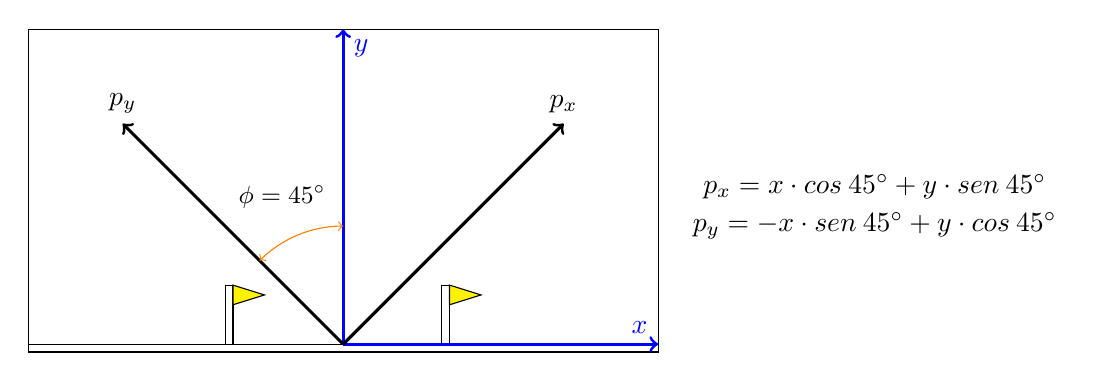
\begin{tikzpicture}
        % Figure 2
        \draw
          (12.25,0) coordinate (a) node[right] {}
        -- (12.25,-3) coordinate (b) node[left] {}
        -- (10.12867,-0.87867) coordinate (c) node[above right] {};
        \draw (8.25,-3) rectangle (16.25,1);
        \draw[fill=white] (8.25, -3) rectangle (16.25,-3.1);
        \draw[fill=white] (10.75, -3) rectangle (10.85,-2.25);
        \draw[fill=yellow] (10.85,-2.5) -- (10.85,-2.25) -- (11.25,-2.375) -- cycle;
        \draw[fill=white] (13.5, -3) rectangle (13.6,-2.25);
        \draw[fill=yellow] (13.6,-2.5) -- (13.6,-2.25) -- (14,-2.375) -- cycle;
        \draw[->, color=blue, line width=1.1pt] (12.25,-3) -- (12.25,1) node[below right] {$y$};
        \draw[->, color=blue, line width=1.1pt] (12.25,-3) -- (16.25,-3) node[above left] {$x$};
        %\node[left] at (16.15,-2.75) {$x$};
        \draw[->, line width=1.1pt] (12.25,-3) -- (9.45,-0.2)node[above] {$p_y$};
        \draw pic["\small $\phi=45^\circ$",draw=orange, <->, angle eccentricity=1.35, angle radius=1.5cm]
        {angle=a--b--c};
        \draw[->, line width=1.1pt] (12.25,-3) -- (15.05,-0.2)node[above] {$p_x$};
        \node at (19, -1) {$ p_x = x\cdot cos\:45^\circ +  y\cdot sen\:45^\circ$};
        \node at (19, -1.5) {$ p_y = -x\cdot sen\:45^\circ +  y\cdot cos\:45^\circ$};
        % Adicione outros detalhes conforme necessário
    \end{tikzpicture}
    \label{fig:enter-label}
\end{figure}

\justifying Com o plano cartesiano rotacionado, é possível estimar três trajetórias de referência.

\end{frame}

%---------------------------------------
% Slide: Modeling Framework
%---------------------------------------

\begin{frame}{\textcolor{blue}{\textbf{GPC: \textit{Lunar Lander}}}}
\vspace{-0.75cm}

\begin{figure}[H]
    \definecolor{rpurple}{RGB}{156, 112, 214}
    \centering
    \vspace*{-.2cm}
    \begin{tikzpicture}
        \draw (7,-3) rectangle (17.5,1);
        \draw[fill=white] (7, -3) rectangle (17.5,-3.1);
        \draw[fill=white] (10.75, -3) rectangle (10.85,-2.25);
        \draw[fill=yellow] (10.85,-2.5) -- (10.85,-2.25) -- (11.25,-2.375) -- cycle;
        \draw[fill=white] (13.5, -3) rectangle (13.6,-2.25);
        \draw[fill=yellow] (13.6,-2.5) -- (13.6,-2.25) -- (14,-2.375) -- cycle;
        \draw[->, line width=1.1pt] (12.25,-3) -- (9.45,-0.2)node[left] {\small $p_y$};
        \draw[->, line width=1.1pt] (12.25,-3) -- (15.05,-0.2)node[right] {\small $p_x$};
        \draw[dashed, line width=1.1pt, color=teal] (12.25,-3) -- (12.25,0.45) node[above]{\footnotesize \textit{Setpoint}: $p_x=p_y$};
        \draw[fill=rpurple, color=rpurple] (11.75,-1)--(12.75,-1)--(12.6,-.5)--(11.9,-.5)-- (11.75,-1);
        \draw[->,line width=1.1pt,  red](12.25,-.75)--(12.25,-1.25);
        \draw[fill=blue] (12.25,-.75) circle (.05); 
        \node at (12.4,-.5)[above right,  line width=1.1pt, color=violet]{\footnotesize \textit{Setpoint}: $\theta =0$};
        \node at (6.935,-.15)[above right,color=red]{\footnotesize \textit{Setpoint}: $v_y = -0,725\cdot p_y - 0,125$};
        % Adicione outros detalhes conforme necessário
    \end{tikzpicture}
    \label{fig:enter-label}
\end{figure}

\justifying Neste contexto lunar, $u$ substitui $\Delta u$ devido à variação na penalização dos propulsores. Quando $h_c < h_p$, $u$ é mantido em 0 para maximizar a recompensa do ambiente.

\end{frame}

%---------------------------------------
% Slide: Modeling Framework
%---------------------------------------

\begin{frame}{\textcolor{blue}{\textbf{GPC: \textit{Lunar Lander}}}}
\vspace{-0.65cm}

\justifying A função de custo para o \textit{Lunar Lander} foi definida como:

\begin{equation}
\label{eq:custogpc}
\begin{matrix}
    J(k) = \sum_{j=d}^{h_p}[\{\alpha\cdot (\hat{p}_x(j+k|k) - \hat{p}_y(j+k|k) )-\beta \cdot \hat{\theta}(j+k|k)\\
            +\delta \cdot  (\hat{v}_y(j+k|k)-0,725\cdot\hat{p}_y(j+k|k)-0,125)\}^2]^\frac{1}{2}\\
\end{matrix}
\end{equation}

\begin{equation*}
\begin{matrix}
  \text{sujeito a:} &  \\
  	Propulsor = & 
  	\left\{
  	\begin{matrix}
  	0 & 0 & 1 & 0\\
       -1  & 0 & 0 & 1 
	\end{matrix} 
	\right\} 
	\begin{matrix}
  	u_1 \Rightarrow\text{Propulsor principal}\\
    u_2 \Rightarrow\text{Propulsor auxiliar}
	\end{matrix}\\
\end{matrix}
\end{equation*}

\justifying Horizonte de controle: 2 ($h_c=2$) e horizonte de predição: 4 ($h_p=4$). Correlação das saídas com entrada específica foram identificadas durante a obtenção do modelo:

\begin{table}[H]
	\centering
	\vspace*{.05cm}
	\begin{tabular}{ccccc}
            \rowcolor{blue!30} Saída & $p_x$ & $\theta$ & $p_y$ & $v_y$ \\
            \hline
            Entrada & $u_2$ & $u_2$ & $u_1$ & $u_1$\\ 
            \hline
	\end{tabular}  
    \label{tab:intcartpole}                 % Nome da tabela para referência cruzada
\end{table}

\end{frame}

%---------------------------------------
% Slide: Modeling Framework
%---------------------------------------

\begin{frame}{\textcolor{blue}{\textbf{GPC: \textit{Lunar Lander}}}}
\vspace{-1.5cm}



\begin{tikzpicture}
  % Desenhe o gráfico
  \draw[->] (2,2) -- (4,4) node[below right] {$p_x$};
  \draw[->] (2,2) -- (0,4) node[below left] {$p_y$};
  
  % Adicione a imagem
  \node at (2,5.5) {
\includegraphics[width=2cm]{images/lander-removebg-preview.png}};
  \draw[->, color=red] (2,5.5) -- (2, 4.25) node[below] {$v_y$};
  \draw[->] (2,5.5) -- (2, 7) node[above] {$N$};
   \draw[fill=blue] (2,5.5) circle (0.05cm);
  \draw[->, color=black] (2,6.67) node[above right]{$\theta$} arc (90:42:0.865cm);
  \node[color=black] at (3.25, 5.5) {$(\textcolor{blue}{p_x}, \textcolor{violet}{p_y})$};
  \node[color=blue] at (8.25, 6.5) {$p_x(k) = 1,9986\cdot p_x(k-1) -0,9986 \cdot p_x(k-2)$};
   \node[color=blue] at (8.35, 6.05) {$-7,3642\cdot 10^{-5}\cdot u_2(k-1) -4,7979\cdot 10^{-4}$};
    \node[color=violet] at (8.4, 5.5) {$p_y(k) = 1,9928\cdot p_y(k-1) - 0,99279\cdot p_y(k-2)$};
    \node[color=violet] at (8.45, 5.05) {$+8,1745\cdot 10^{-5}\cdot u_1(k-1) -3,9457\cdot 10^{-4}$};
    \node[color=black] at (8.12, 7.5) {$ \theta(k) = -1,9891\cdot \theta(k-1) +0,989\cdot \theta(k-2)$};
    \node[color=black] at (8.45, 7.05) {$+1,7201\cdot 10^{-4}\cdot u_2(k-1)$};
   \node[color=red] at (8.35, 4.5) {$v_y(k) = 1,2503\cdot v_y(k-1) - 0,25137\cdot v_y(k-2)$};
    \node[color=red] at (8.7, 4.05) {$-1,3791\cdot 10^{-2}\cdot u_1(k-1)+2,3644\cdot 10^{-3}$};
    \node[color=black] at (0, 9) {};
    \draw[fill=brown!35] (-1,2) rectangle (5,1.9);
    \draw[fill=white] (-.25, 2) rectangle (-.35,2.75);
    \draw[fill=yellow] (-.25,2.5) -- (-.25,2.75) -- (0.05,2.625) -- cycle;
    \draw[fill=white] (4.25, 2) rectangle (4.15,2.75);
    \draw[fill=yellow] (4.25,2.5) -- (4.25,2.75) -- (4.55,2.625) -- cycle;
\end{tikzpicture}

\end{frame}

%---------------------------------------
% Slide: Modeling Framework
%---------------------------------------

\begin{frame}{\textcolor{blue}{\textbf{GPC: \textit{Lunar Lander}}}}
\vspace{-.15cm}

\justifying Pesos utilizados:

\begin{figure}[H]
    \definecolor{rpurple}{RGB}{156, 112, 214}
    \centering
    \vspace*{-.05cm}
    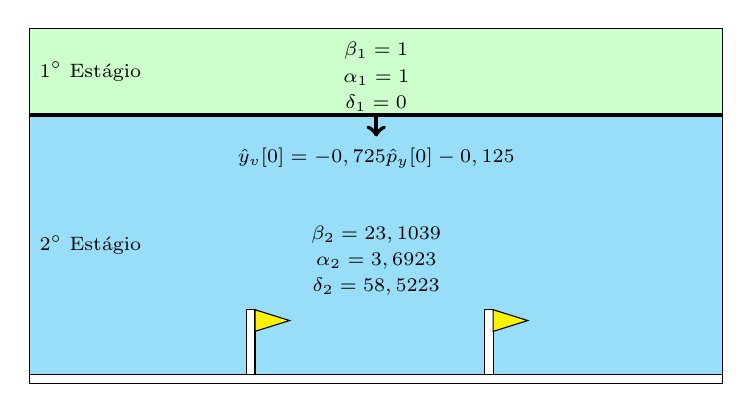
\begin{tikzpicture}[scale=1.1]
        \draw[fill=green!60] (8.25,0) rectangle (16.25,1);
        \draw[fill=cyan!40] (8.25,0) rectangle (16.25,-3);
        \draw (8.25,-3) rectangle (16.25,1);
        \draw[fill=green!20] (8.25,0) rectangle (16.25,1);
        \draw[fill=white] (8.25, -3) rectangle (16.25,-3.1);
        \draw[fill=white] (10.75, -3) rectangle (10.85,-2.25);
        \draw[fill=yellow] (10.85,-2.5) -- (10.85,-2.25) -- (11.25,-2.375) -- cycle;
        \draw[fill=white] (13.5, -3) rectangle (13.6,-2.25);
        \draw[fill=yellow] (13.6,-2.5) -- (13.6,-2.25) -- (14,-2.375) -- cycle;
        \draw[color=black, line width=1.5pt] (8.25,0) -- (16.25,0);
        \node at (12.25,.53)[above]{\scriptsize $\beta_1 = 1$};
        \node at (12.25,.23)[above]{\scriptsize $\alpha_1 = 1$};
        \node at (12.25,-.07)[above]{\scriptsize $\delta_1 = 0$};
        \node at (12.25,-1.6)[above]{\scriptsize $\beta_2 = 23,1039$};
        \node at (12.25,-1.9)[above]{\scriptsize $\alpha_2 = 3,6923$};
        \node at (12.25,-2.2)[above]{\scriptsize $\delta_2 = 58,5223$};
        \node at (8.25,.5)[right]{\scriptsize $1^\circ$ Estágio};
        \node at (8.25,-1.5)[right]{\scriptsize $2^\circ$ Estágio};
        \draw[->, color=black,  line width=1.5pt](12.25,0)--(12.25,-.25) node[below]{\scriptsize $\hat{y}_v[0]=-0,725\hat{p}_y[0]-0,125$};;
        % Adicione outros detalhes conforme necessário
    \end{tikzpicture}
    \label{fig:enter-label}
\end{figure}
\vspace{1cm}
\end{frame}

%%%%%%%%%%%%%%%%%%%%%%%%%%%%%%%%%%%%%%%%
% Section: Results 
%%%%%%%%%%%%%%%%%%%%%%%%%%%%%%%%%%%%%%%%
\section{\textbf{\textcolor{purple}{Resultados}}}
    \begin{frame}[plain]
        \vfill
      \centering
      \begin{beamercolorbox}[sep=8pt,center,shadow=true,rounded=true]{title}
        \usebeamerfont{title}\insertsectionhead\par%
        \color{oxfordblue}\noindent\rule{10cm}{1pt}
      \end{beamercolorbox}
      \vfill
  \end{frame}

%---------------------------------------
% Slide: Model Results
%---------------------------------------
\begin{frame}{\textcolor{blue}{\textbf{\textit{Cart Pole}}}}
\vspace{-.75cm}
\begin{minipage}{0.5\textwidth}
  \centering
  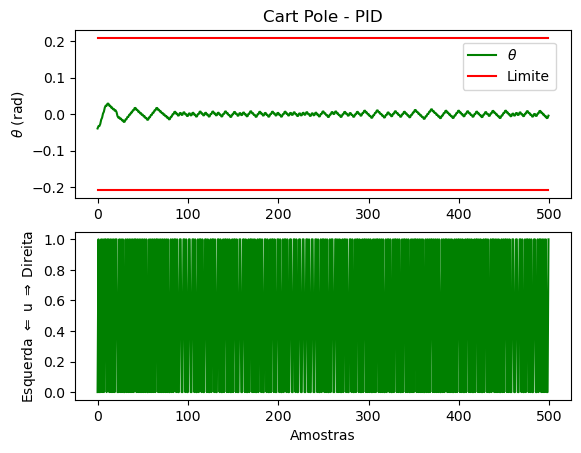
\includegraphics[scale=0.45]{images/ctpidio.png}
  \label{fig:imagem1}
\end{minipage}%
\begin{minipage}{0.5\textwidth}
  \centering
  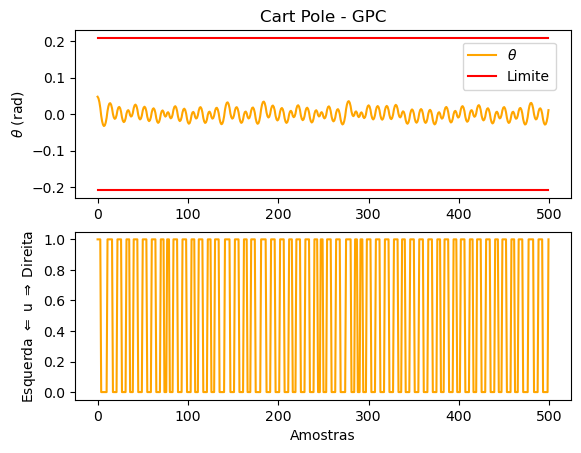
\includegraphics[scale=0.45]{images/ctgpcio.png}
  \label{fig:imagem2}
\end{minipage}

\begin{table}[H]
	\centering
	\vspace*{-.2cm}
	\begin{tabular}{ccccc}
            \rowcolor{blue!30} Controle & $\bar{\theta}$ & $\theta_{max}$ & Etapas & Tempo de Execução $[s]$\\
            \hline
            PID & $1,1053\cdot 10^{-5}$ & $4,6395\cdot 10^{-2}$ & 5000 & $9,0421$\\
            GPC & $-9,7546\cdot 10^{-5}$ & $7,3337\cdot 10^{-2}$  & 5000 & $15,1423$\\ 
            \hline
	\end{tabular}  
    \label{tab:intcartpole}                 % Nome da tabela para referência cruzada
\end{table}

\end{frame}

%---------------------------------------
% Slide: Model Results
%---------------------------------------

\begin{frame}{\textcolor{blue}{\textbf{\textit{Lunar Lander}}}}
\vspace{-.75cm}
\begin{minipage}{0.5\textwidth}
  \centering
  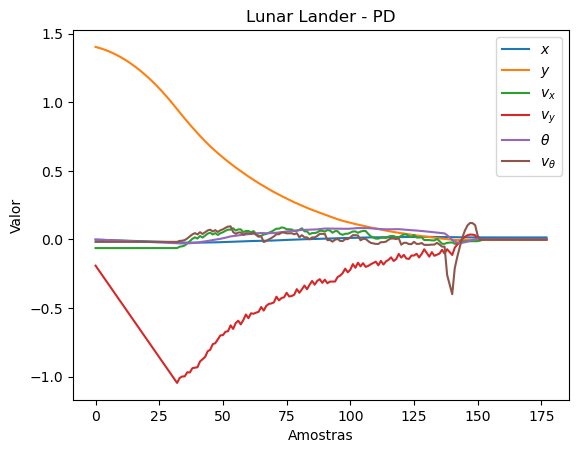
\includegraphics[scale=0.45]{images/llpid.png}
  \label{fig:imagem1}
\end{minipage}%
\begin{minipage}{0.5\textwidth}
  \centering
  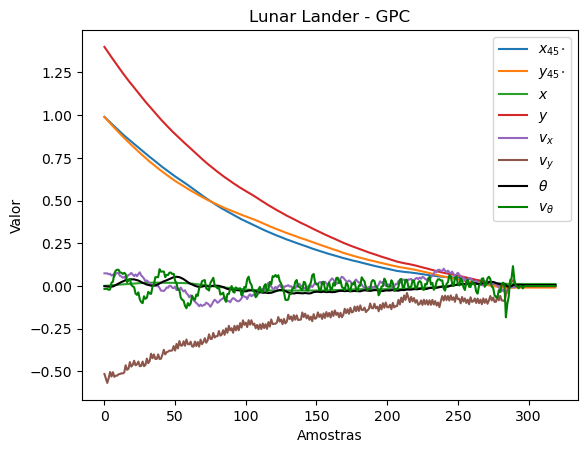
\includegraphics[scale=0.45]{images/llgpc.png}
  \label{fig:imagem2}
\end{minipage}

\begin{table}[H]
	\centering
	\vspace*{-.2cm}
	\begin{tabular}{cccccc}
              \rowcolor{blue!30} Controle & Pouso & Pouso com +200 pontos & Etapas & Tempo [$s$] & Média\\
            \hline
            PD & $765$ & $764$ &  $177577$ & $1086,6976$ & $217,4862$\\
            GPC & $870$ & $808$  &  $340369$ & $1017,0346$ & $209,1881$\\ 
            \hline
	\end{tabular}  
    \label{tab:intll}                 % Nome da tabela para referência cruzada
\end{table}


\end{frame}

%%%%%%%%%%%%%%%%%%%%%%%%%%%%%%%%%%%%%%%%
% Section: Study Conclusions, Contributions, and Practical Implications 
%%%%%%%%%%%%%%%%%%%%%%%%%%%%%%%%%%%%%%%%
\section{\textbf{\textcolor{purple}{Conclusão}}}
    \begin{frame}[plain]
        \vfill
      \centering
      \begin{beamercolorbox}[sep=8pt,center,shadow=true,rounded=true]{title}
        \usebeamerfont{title}\insertsectionhead\par%
        \color{oxfordblue}\noindent\rule{10cm}{1pt}
      \end{beamercolorbox}
      \vfill
  \end{frame}

%---------------------------------------
% Slide: Study Conclusions
%---------------------------------------

\begin{frame}{\textcolor{blue}{\textbf{Conclusões do Estudo}}}
\begin{itemize}
    \justifying 
    \item[\textcolor{blue}{\checkmark}]   Ambos os controladores demonstraram eficácia no controle tanto do \textit{Cart Pole} quanto do \textit{Lunar Lander};
    \item[\textcolor{blue}{\checkmark}]  O controlador PID destacou-se pela sua eficácia no \textit{Cart Pole}, enquanto o GPC mostrou-se mais eficiente no \textit{Lunar Lander};
    \item[\textcolor{blue}{\checkmark}] Este trabalho revelou especificidades distintas de cada técnica, oferecendo uma aplicação prática e comparativa entre elas.
\end{itemize}
\end{frame}

%%%%%%%%%%%%%%%%%%%%%%%%%%%%%%%%%%%%%%%%
% Section: References 
%%%%%%%%%%%%%%%%%%%%%%%%%%%%%%%%%%%%%%%%



%\section{Bibliography}
\section{\textbf{\textcolor{purple}{Referências Bibliográficas}}}
\begin{frame}[allowframebreaks]
  \frametitle{Referências Bibliográficas}
  \bibliographystyle{IEEEtran}
  \bibliography{references.bib}
  \nocite{*}
\end{frame}


%%%%%%%%%%%%%%%%%%%%%%%%%%%%%%%%%%%%%%%%
% Slide: Last Slide 
%%%%%%%%%%%%%%%%%%%%%%%%%%%%%%%%%%%%%%%%
\begin{frame}{}
    \begin{center}
        \vspace{10mm}
        \textbf{\textcolor{teal!80}{\huge Muito Obrigado!}}
    \end{center}
\end{frame}

\end{document}
